% Figure: t-SNE of ConvNeXt-Tiny pre-logit features, Task B test split
% Source   : artifact/person1/tsne/  (repo ManifoldsTeam/WoodID, branch p1,
%            commit d39a3f6b2cc5942e1e718c0dca86e89b0d81eb4d; see SOURCE.txt)
% Run id   : taskB17__main__seed_42__convnext_tiny  (same registry as Table 1)
% Artifacts: features_convnext_seed42_test.npz, tsne_embedding.csv,
%            tsne_metadata.json
\begin{figure}[!htbp]
\centering
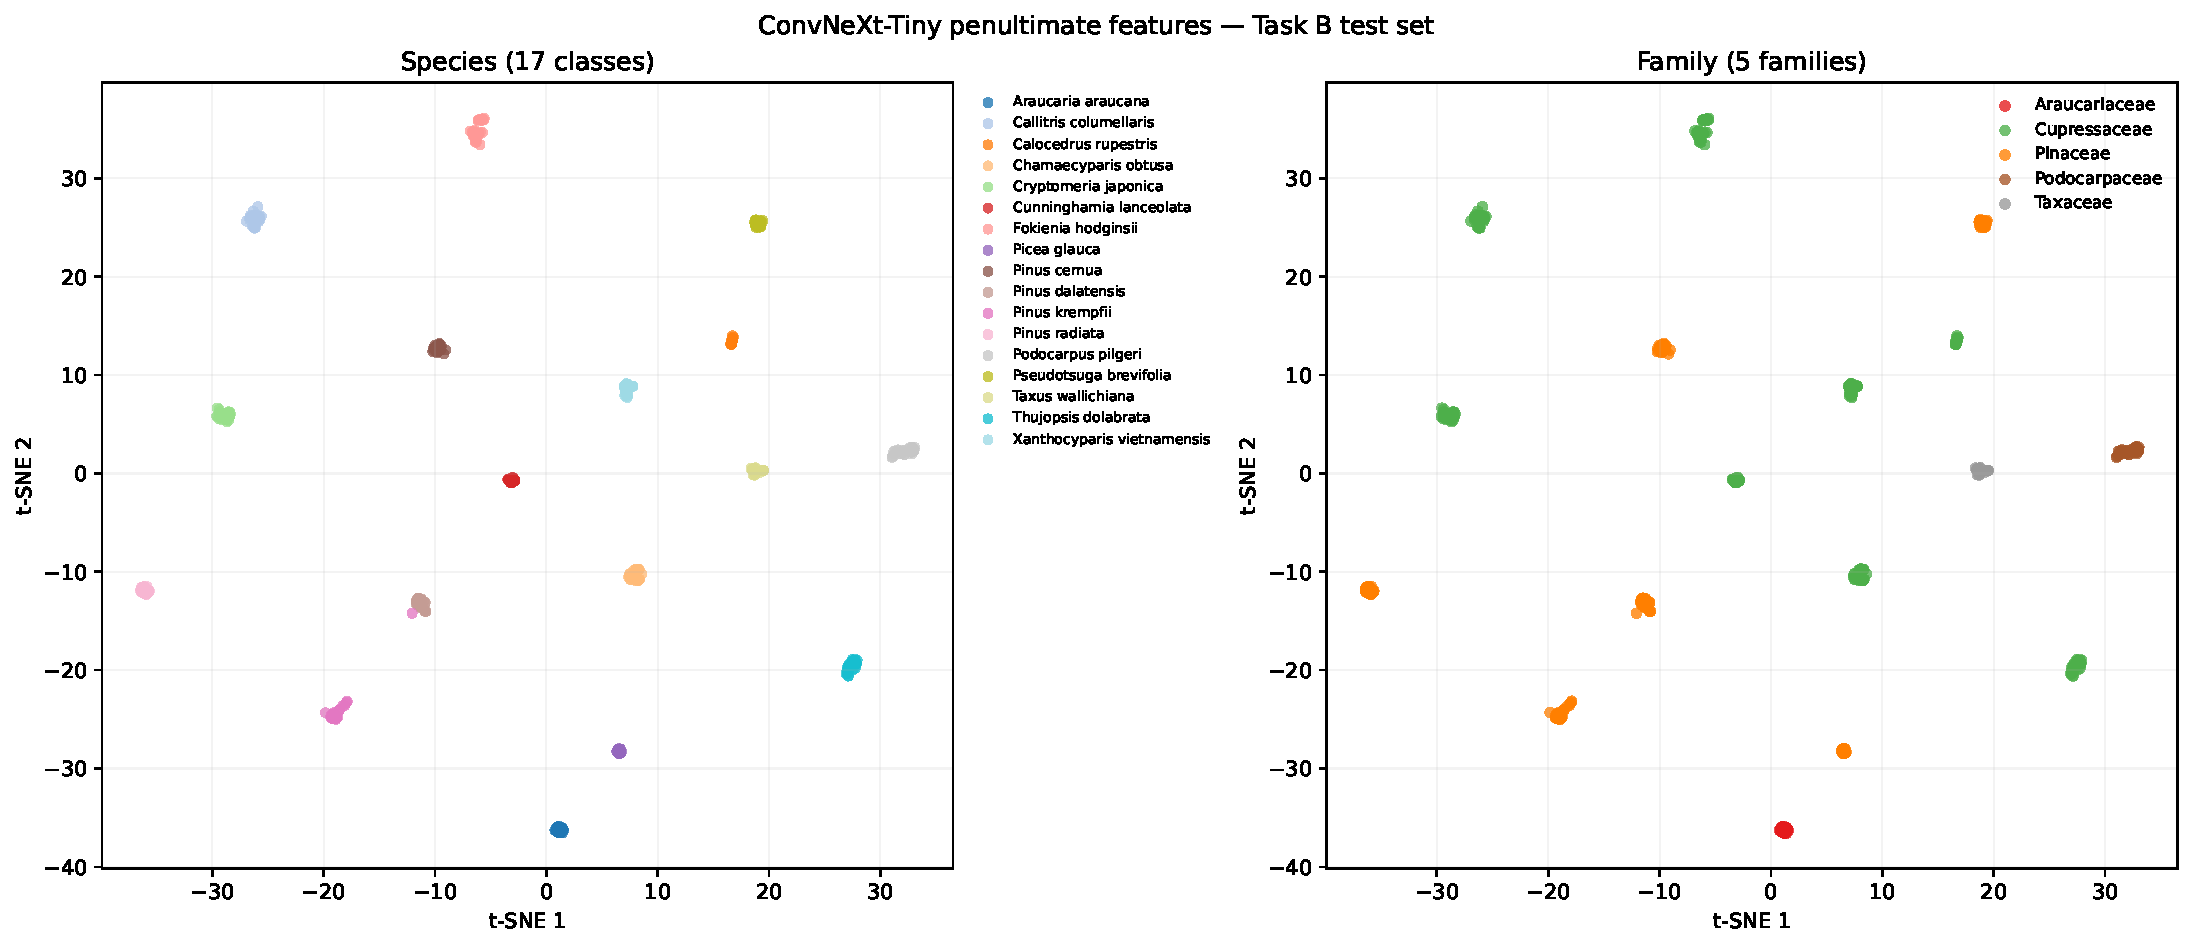
\includegraphics[width=\linewidth]{artifact/person1/tsne/fig_tsne.pdf}
\caption{Phép nhúng t-SNE hai chiều của đặc trưng ConvNeXt-Tiny cho cả 532 ảnh test Task~B, lấy từ lần chạy seed 42 ở Bảng~\ref{tab:task_b}. Đặc trưng là kích hoạt 768 chiều trước lớp logit, được chuẩn hóa, giảm xuống 50 chiều bằng PCA rồi xuống hai chiều bằng t-SNE với perplexity 30, khởi tạo PCA và seed ngẫu nhiên cố định. t-SNE chỉ bảo toàn láng giềng cục bộ: khoảng cách và diện tích cụm trong hình không phải metric, và phép nhúng được trình bày như một cách nhìn định tính về biểu diễn chứ không phải bằng chứng về tính tách được.}
\label{fig:tsne}
\end{figure}
